% DO NOT COMPILE THIS FILE DIRECTLY!
% This is included by the other .tex files.


\begin{frame}
    
\includegraphics[scale=.3]{images/logo-circl-Forensics.png}
    \begin{itemize}
        \item[]
        \item[]
        \item[] 14. Event Logs
    \end{itemize}
\end{frame}


\begin{frame}[fragile]
  \frametitle{14.1 Overview: Windows Event Logs}
    \begin{itemize}
        \item Up to Windows XP
            \begin{itemize}
                \item Binary Event Log file format
                \item Mainly 3 categories:
                \begin{itemize}
			\item[] Security
			\item[] System
			\item[] Application
			\item[] ... some server service specific
			\item[]
                \end{itemize}
            \end{itemize}
        \item Beginning with Vista
            \begin{itemize}
		\item New extension: \texttt{.evtx}
                \item New format based on XML
		\item Location: \texttt{/Windows/System32/winevt/Logs/}
                \item Many more files:
                \begin{itemize}
			\item[] Security
			\item[] System
			\item[] Application
			\item[] \texttt{\$ ls | wc -l}
			\item[] \texttt{59}
                \end{itemize}
            \end{itemize}
    \end{itemize}
\end{frame}


\begin{frame}[fragile]
  \frametitle{14.1 Overview: Windows Event Logs}
    \begin{itemize}
        \item Review logging policies
  \begin{lstlisting}[basicstyle=\tiny]
$ rip.pl -r SECURITY -p auditpol
.....
ystem:Other System Events                         S/F  
Logon/Logoff:Logon                                 S    
Logon/Logoff:Logoff                                S    
Logon/Logoff:Account Lockout                       S    
Logon/Logoff:IPsec Main Mode                       N    
Logon/Logoff:IPsec Quick Mode                      S    
Logon/Logoff:IPsec Extended Mode                   N    
Logon/Logoff:Special Logon                         N    
Logon/Logoff:Other Logon/Logoff Events             N    
Logon/Logoff:Network Policy Server                 S/F  
Object Access:File System                          N    
.....
  \end{lstlisting}
        \item Get details online:
            \begin{itemize}
                \item Microsoft TechNet
		\item \url{https://www.ultimatewindowssecurity.com/securitylog/encyclopedia/}
		\item \url{http://eventid.net/}
            \end{itemize}
    \end{itemize}
\end{frame}


\begin{frame}[fragile]
  \frametitle{14.2 Example: Login}
    \begin{itemize}
        \item Succsessful
  \begin{lstlisting}[basicstyle=\tiny]
$ evtxexport Security.evtx | less
.....
Event number          : 668
Written time          : Apr 15, 2019 12:58:33.650031000 UTC
Event level           : Information (0)
Computer name         : Win7WS
Source name           : Microsoft-Windows-Security-Auditing
Event identifier      : 0x00001210 (4624)
Number of strings     : 20
String: 1             : S-1-5-18
String: 2             : WIN7WS$
String: 3             : WORKGROUP
String: 4             : 0x00000000000003e7
String: 5             : S-1-5-21-3408732720-2018246097-660081352-1000
String: 6             : John
String: 7             : Win7WS
String: 9             : 2
.....
String: 17            : 0x0000018c
String: 18            : C:\Windows\System32\winlogon.exe
String: 19            : 127.0.0.1
  \end{lstlisting}
        \item Failed
  \begin{lstlisting}[basicstyle=\tiny]
$ evtxexport Security.evtx | grep 4625
  \end{lstlisting}
    \end{itemize}
\end{frame}


\begin{frame}[fragile]
  \frametitle{14.2 Example: Login}
    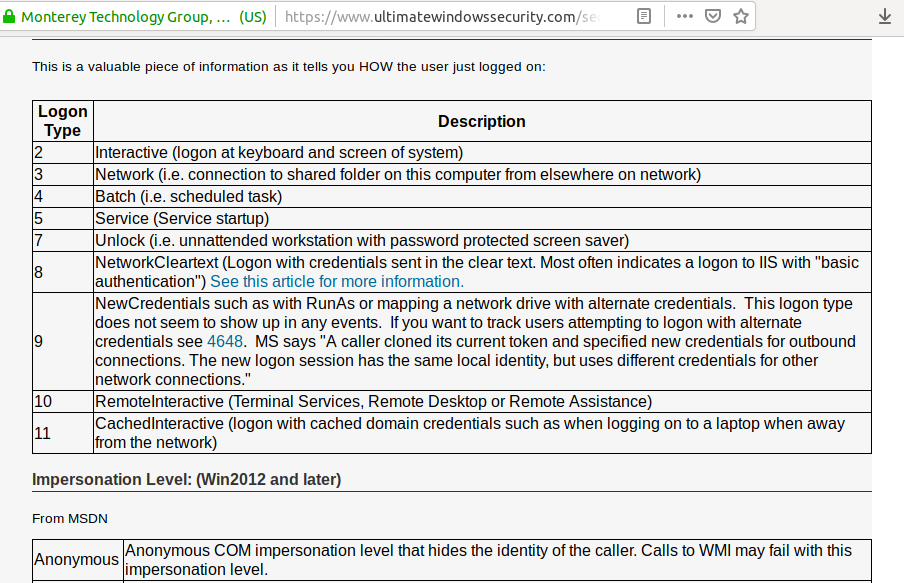
\includegraphics[scale=0.4]{images/f14_logonType.png}
\end{frame}


\begin{frame}[fragile]
  \frametitle{14.3 Other log files}
    \begin{itemize}
	\item \texttt{/Windows/setuplog.txt}
        \begin{itemize}
            \item Untill WinXP, when Windows is installed
        \end{itemize}
	\item \texttt{/Windows//Debug/netsetup.log}
        \begin{itemize}
            \item Untill WinXP, when Windows is installed
        \end{itemize}
	\item \texttt{/Windows/setupact.log}
        \begin{itemize}
            \item Graphical part of setup process
  \begin{lstlisting}[basicstyle=\tiny]
2019-04-05 11:39:56, Info  CBS Starting the TrustedInstaller main loop.
2019-04-05 11:39:56, Info  CBS TrustedInstaller service starts successfully.
2019-04-05 11:39:56, Info  CBS Setup in progress, aborting startup processing checks.
2019-04-05 11:39:56, Info  CBS Startup processing thread terminated normally
    \end{lstlisting}
	\end{itemize}
	\item \texttt{/Windows/setupapi.log}
  \begin{lstlisting}[basicstyle=\tiny]
/Windows/inf/setupapi.dev.log
/Windows/inf/setupapi.app.log
/Windows/inf/setupapi.offline.log
    \end{lstlisting}
	\item \texttt{/Windows/Tasks/SCHEDLGU.TXT}
        \begin{itemize}
            \item Task Scheduler Log
	\end{itemize}
    \end{itemize}
\end{frame}


\begin{frame}[fragile]
  \frametitle{14.4 Event Logs: Exercise}
    \begin{enumerate}
        \item Which .evtx files could be interesting for forensics?
        \item Extract promising .evtx files
	\item Try tools like \texttt{evtx\_dump.py} to read some logs
        \item Find general information like:
        \begin{itemize}
            \item What time the system boot up
            \item What user was logged on
            \item Was there much user activity before infection
            \item What time the system shut down
        \end{itemize}
        \item Search for other incident related artefacts in .evtx files
        \item Are artefacts within the other log files?
    \end{enumerate}
\end{frame}





